\documentclass[11pt]{article}

%% Separate file for preamble with macros and stuff
\usepackage[T1]{fontenc}
\usepackage[a4paper, top=1in, bottom=1.1in, left=1in, right=1in]{geometry}
\usepackage[toc,page]{appendix}
\usepackage[utf8]{inputenc} % utf8
\usepackage{amsmath}
\usepackage{attachfile}
\usepackage{booktabs}
\usepackage{caption}
\usepackage{commath}
\usepackage{graphicx}
\usepackage{hyperref}
\usepackage{listings}
\usepackage{mathtools}
\usepackage{siunitx}
\usepackage{subcaption}
\usepackage{tabularx}
\usepackage{url}
\usepackage{varioref}
\usepackage{wrapfig}
\usepackage{xcolor}

\setlength{\belowcaptionskip}{-6pt}
\makeatletter
\lst@Key{matchrangestart}{f}{\lstKV@SetIf{#1}\lst@ifmatchrangestart}
\def\lst@SkipToFirst{%
  \lst@ifmatchrangestart\c@lstnumber=\numexpr-1+\lst@firstline\fi
  \ifnum \lst@lineno<\lst@firstline
  \def\lst@next{\lst@BeginDropInput\lst@Pmode
    \lst@Let{13}\lst@MSkipToFirst
    \lst@Let{10}\lst@MSkipToFirst}%
  \expandafter\lst@next
  \else
  \expandafter\lst@BOLGobble
  \fi}
\makeatother

\lstset{  
  backgroundcolor=\color{gray!30},   % choose the background color; you must add \usepackage{color} or \usepackage{xcolor}
  basicstyle=\scriptsize,        % the size of the fonts that are used for the code
  breakatwhitespace=false,         % sets if automatic breaks should only happen at whitespace
  breaklines=true,                 % sets automatic line breaking
  captionpos=t,                    % sets the caption-position to bottom
  escapeinside={\%*}{*)},          % if you want to add LaTeX within your code
  extendedchars=true,              % lets you use non-ASCII characters; for 8-bits encodings only, does not work with UTF-8
  frame=single,                   % adds a frame around the code
  keepspaces=true,                 % keeps spaces in text, useful for keeping indentation of code (possibly needs columns=flexible)
  keywordstyle=\color{blue},       % keyword style
  language=C++,                 % the language of the code
  numbers=left,                    % where to put the line-numbers; possible values are (none, left, right)
  numbersep=20pt,                   % how far the line-numbers are from the code
  numberstyle=\tiny\color{gray}, % the style that is used for the line-numbers
  rulecolor=\color{blue!20},       
  showspaces=false,                % show spaces everywhere adding particular underscores; it overrides 'showstringspaces'
  showstringspaces=false,          % underline spaces within strings only
  showtabs=false,                  % show tabs within strings adding particular underscores
  stepnumber=1,                    % the step between two line-numbers. If it's 1, each line will be numbered
  tabsize=2,                   % sets default tabsize to 2 spaces
  framesep=7pt,
  xleftmargin=12pt,
  xrightmargin=11pt
}


\setlength{\fboxsep}{4pt}
\DeclareCaptionFormat{myformat}{%
  \hspace{1pt}\fcolorbox{blue!20}{gray!20}{\footnotesize\parbox{\dimexpr\textwidth-17pt\relax}{#1#2\ttfamily#3}}\vspace{-4pt}
}
\captionsetup[lstlisting]{format=myformat}

\captionsetup[figure]{labelfont=sf,hypcap=false,format=hang,margin=0.5cm,justification=RaggedRight,calcwidth=0.7\linewidth,font=footnotesize,justification=justified}
\captionsetup[subfigure]{labelfont=sf,hypcap=false,format=hang,margin=0.5cm,justification=RaggedRight,calcwidth=0.7\linewidth,font=footnotesize,justification=justified}
\captionsetup[table]{labelfont=sf,hypcap=false,format=hang,margin=1cm,justification=RaggedRight,calcwidth=0.8\linewidth,font=footnotesize,justification=justified}
\labelformat{equation}{(#1)}

%%% Math typesetting macros
\newcommand{\di}[2]{#1_\textup{#2}} % Descriptive Index: Macro for quick upright index (as opposed to a variable index, which should be italic)


\renewcommand{\lstlistlistingname}{Code listings}
\bibliographystyle{ieeetr}


%%%%%%%%%%%%%%%%%%%%%%%%%%%%%%
%%% STOLEN FROM STACKOVERFLOW
%%%%%%%%%%%%%%%%%%%%%%%%%%%%%%

\newcommand\YAMLcolonstyle{\color{red}\mdseries\scriptsize}
\newcommand\YAMLkeystyle{\color{black}\bfseries\scriptsize}
\newcommand\YAMLvaluestyle{\color{blue}\mdseries\scriptsize}

\makeatletter

% here is a macro expanding to the name of the language
% (handy if you decide to change it further down the road)
\newcommand\language@yaml{yaml}

\expandafter\expandafter\expandafter\lstdefinelanguage
\expandafter{\language@yaml}
{
  keywords={true,false,null,y,n},
  keywordstyle=\color{darkgray}\bfseries,
  basicstyle=\YAMLkeystyle,                                 % assuming a key comes first
  sensitive=false,
  comment=[l]{\#},
  morecomment=[s]{/*}{*/},
  commentstyle=\color{purple}\ttfamily,
  stringstyle=\YAMLvaluestyle\ttfamily,
  moredelim=[l][\color{orange}]{\&},
  moredelim=[l][\color{magenta}]{*},
  moredelim=**[il][\YAMLcolonstyle{:}\YAMLvaluestyle]{:},   % switch to value style at :
  morestring=[b]',
  morestring=[b]'',
  literate =    {---}{{\ProcessThreeDashes}}3
  {>}{{\textcolor{red}\textgreater}}1
  {|}{{\textcolor{red}\textbar}}1
  {\ -\ }{{\mdseries\ -\ }}3,
}

% switch to key style at EOL
\lst@AddToHook{EveryLine}{\ifx\lst@language\language@yaml\YAMLkeystyle\fi}
\makeatother

\newcommand\ProcessThreeDashes{\llap{\color{cyan}\mdseries-{-}-}}


\renewcommand{\tabularxcolumn}[1]{>{\small}m{#1}}
%%% Local Variables:
%%% mode: latex
%%% TeX-master: t
%%% End:
 

%% For make-title
\title{Laboration 2: RGBD-cameras\\ {\small Sensors and Sensing}}
\author{Marek Bečica, Tom Olsson}
\date{\today}

\begin{document}
\maketitle %Title area
\begin{center}
  \emph{All code for this exercise can be found at \\ \url{https://github.com/tgolsson/sensors-laboration2-xtion}}
\end{center}
\tableofcontents
\lstlistoflistings % List of all code snippets
\listoffigures % List of all figures
\listoftables
\lstset{ matchrangestart=t} %initialise the linerange-macro for \lstinput...
\section{Theory and motivation}
\subsection{RGBD-cameras}
RGBD-cameras, short for \emph{Red-Green-Blue-Depth}-camera, is a type of low-cost camera commonly used for robot vision. The concept became widely popular with the release of the Microsoft Kinect in late 2010. \par

These cameras consist of two separate parts: one normal color-based camera, and one infra-red sensor with accompanying projector. The sensing consists of projecting a deterministic pattern onto the scene using an infrared emitter, and then unprojecting by comparing the image to previously captured patterns at known depths. By interpolating through these patterns, a full depth-image is generated.  
\subsection{Noise}

A common problem in any type of sensing is the introduction of noise into the system. This noise can come from many sources, and be predictable or unpredictable. Examples of noise sources could be frequency hum from electric circuits, flickering lights, air pollution or pure inaccuracy. This noise can skew the results of sensors that make algorithm much more error prone. \par

There are many approaches to reduce noise. Proper calibration and good testing environments is a good start, but this can only reduce external noise. Internal noise of the sensor needs to be analyzed and minimized on a much lower-level such as by using specially constructed algorithms. For sensors that generate some sort of sequence, one very naive (but nonetheless effective) approach is the use of smoothing. \par

\section{Implementation}
The purpose of this exercise is to calibrate an RGBD-camera and investigate its characteristics. Then, several smoothing algorithms shall be evaluated to reduce noise in the depth sensor.
\subsection{Hardware and environment}
This exercise was performed using an \emph{ASUS Xtion Pro}. The camera was connected over \emph{USB2} to a laptop running Linux kernel 4.2.5. The communication to the camera is done using the \emph{Robot Operating System} [ROS] version \emph{Indigo Igloo}. All ROS packages used are compiled directly from GitHub development branch for Indigo Igloo. \par
Other software used includes the OpenCV libraries, version 2.4.12.2-1.
\subsection{Camera setup}
% TODO: Marek : Screenshots, short introduction
As a first step we had to install \emph{openni2} package for the corresponding version of ROS. This package contains drivers for the Asus camera. After installing the package we connected the camera to the USB 2.0 port on the laptop. We made sure that our system can recognize the camera through command \emph{lsusb} and after that we run the openi2 package using \texttt{roslaunch openni2\_launch openni2.launch}. During the first launch there was a warning about no calibration file found, but we didn't need it yet for the camera testing. After running openni2 we run in the new terminal window command \texttt{rosrun rviz rviz}, which we used for inspecting the topics where camera publishes its data. In the RVIZ window we need to set global option \textbf{Fixed Frame} to \textbf{camera\_link} in order to see the camera data. \par

We need to create several visualizations to see what camera publishes on each topic. There are four major types of topics with different subtopics that can be visualized using RVIZ. There are topics for \textbf{depth image}, \textbf{depth registered image}, \textbf{RGB image} and \textbf{infrared image}.  The topics can be seen in table \vref{tab:table1}. \par
\begin{table}[h!]
  \centering
  \caption{Camera ROS topics}
  \label{tab:table1}
  \begin{tabular}{ccc}
    \toprule
    Topic & Description & Data preview\\
    \midrule
    topic & info & preview\\
    topic & info & preview\\
    topic & info & preview\\
    topic & info & preview\\
    topic & info & preview\\
    topic & info & preview\\
    \bottomrule
  \end{tabular}
\end{table}
\subsection{ROS setup}
Instead of using RVIZ to view the data as before, a custom ROS-node can be used. As there are three types of data - color image, depth image, and pointcloud, there are three listeners setup to receive this data. An example of the data on these topics can be found in the embedded files below\footnote{If these embedded files do not work, such as if you use Adobe Acrobat, please download them from the \texttt{report} folder in the GitHub repository. Verified to work with Okular and Evince on Linux.}. The \texttt{depth image} and \texttt{color image} are stored in the OpenCV \texttt{y[a]ml} format, and the point cloud is stored in the \emph{Point Cloud Library} [PCL] \texttt{pcd} format.\par

\begin{center}
  \attachfile[color=0 0 0,icon=Paperclip]{pcloud.pcd}{{  }Pointcloud file}{   }
  \attachfile[color=0 0 0,icon=Paperclip]{rgbbmp.yml}{{  }RGB-image file}{   }
  % \attachfile[color=0 0 0, icon=Paperclip]{depthimage.yml}{Depth-image file}
\end{center}

\subsection{Camera calibration}
% TODO: Marek : Calibration file & process
	In this part we were supposed to calibrate the camera which requires to setup internal parameters. After that we should be able to get not distorted image from the camera and right distance measurement. \par

	As a first step we had to install \emph{camera\_calibration} package. After that we listed all topics where camera publishes its data and we choosed topic \texttt{/camera/rgb/image\_raw}. Before running calibration process, we need to measure how many squares are in the checkerboard pattern and what is the length of one square. Using the command \texttt{rosrun camera\_calibration cameracalibrator.py --size=6x10 --square=0.065 image:=/camera/rgb/image\_raw{ }}\texttt{camera:=/camera/rgb --approximate=0.1}, we run the calibration application with correctly setup parameters according to our measurements of the calibrating pattern. In the calibration window we could see image from the selected topic with detection of the pattern. We set the camera to the parallel position with the ground and pointed it to the wall. After that we kept moving and tilting the pattern all over the camera field of view until X, Y and Size progressbar showed long line and button Calibrate light up. This process took up about 2 minutes until we got good results and Calibration button lighted up. We pressed the button and then waited for few minutes until the application was able to compute the right parameters for our camera. After that buttons Save and Upload lighted up. We saved the calibration file and tried to upload it to the camera firmware, but for some reason that function didn't worked properly and we had to set the calibration file as a parameter of the openni2 package. The calibration file was saved into \emph{out.txt} file in the tmp directory and we needed to convert it to yaml file. In order to do that, we used command \texttt{rosrun camera\_calibration\_parsers convert  out.txt camera.yaml} which converted the calibration file into yaml file which we could use for the openni2 package. The calibration file is shown in listing \vref{lst:calib}. \par
	To check the calibration results we tried to point the camera at some straight lines (wall corners, table etc.) and checked if they got distorted around the edges. That showed that the straight lines stayed as a straight lines, so the calibration was successful. To verify if the calibration worked in the quantitative manner we run the code from the Task 4: Noise characterization, that measured average and standard deviation for the distance in the small window. Then we pointed the camera to the objects in different distances and checked if the mean of the distance is the same as the reality, which mostly was within the range of the camera. \par
	
\lstinputlisting[language=yaml,caption={The calibration file for the camera}, label={lst:calib}]{camera.yaml} 

\subsection{Noise characterization}
The sensors used in the camera suffer from noise, and the first requirement for improvement is to objectively quantify the error. First, 5 measurements of 10 seconds each were recorded with \texttt{rosbag}. The measurements were taken \emph{50}, \emph{100}, \emph{150}, \emph{200}, and \emph{300} cm from a white wall. The camera was placed on a table, so that the  camera normal was perpendicular to the wall. This ensures that all measurements are made against the same baseline. \par

First, the errors were quantified at varying distance with set window sizes. Fig. \vref{fig:20x20} shows the error and variances for a 20x20 window, and fig. \vref{fig:40x40} shows the same for a 40x40 window. The most obvious pattern can be seen in the left-most plot in the two figures: there is a very strong correlation between distance and both variance and error. This has been shown by other researchers, and is logical: the further the distance, the more things can interfere with measurements such as light conditions, dust particles, and so on. \par

Another interesting pattern is that the mean error barely changes between the two windows; however, a larger window reduces the variance significantly. This is not so much related to reduced errors, but a result of the definition of a variance. If the errors are assumed to adhere to some sort of distribution $X \in \left(-\infty, \infty \right)$, then $\sum_{X_1}^{X_\infty} = \bar{X}$, i.e., the static error. From this it follows that the variance will then also be the pure noise in the signal. However, if too few points are sampled the sum will only approximate the mean, and the variance will become unstable.


\begin{figure}[ht]
  \centering
  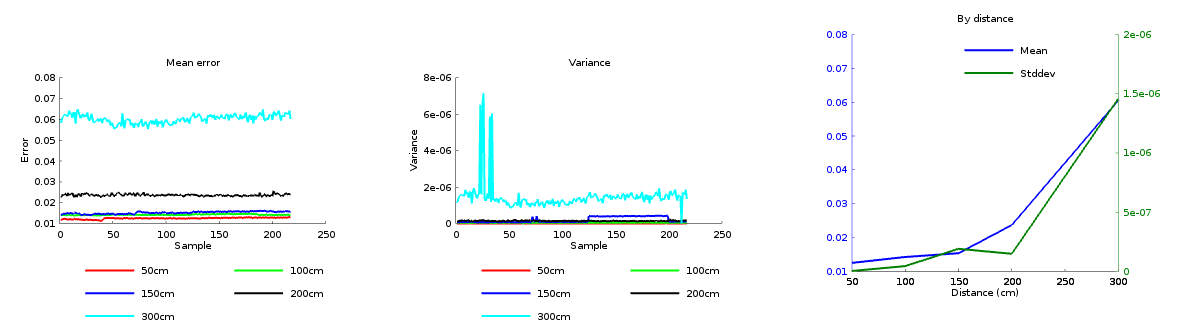
\includegraphics[width=1\textwidth]{figures/20x20-plot.png}
  \captionof{figure}[Mean and variance: 20x20 window]{\label{fig:20x20} The error and variance for a 20x20 pixel window at the center.}
\end{figure}
\begin{figure}[ht]
  \centering
  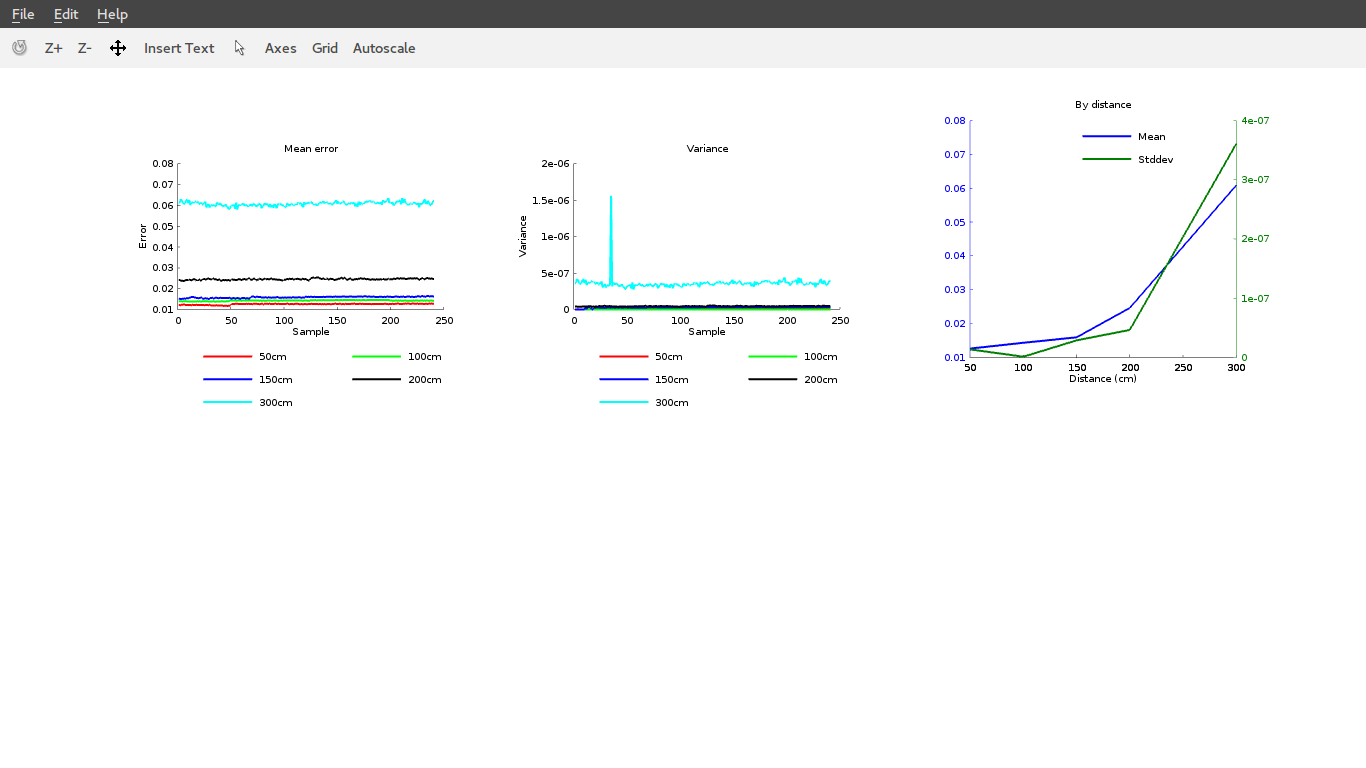
\includegraphics[width=1\textwidth]{figures/plot40x40.png}
  \captionof{figure}[Mean and variance: 40x40 window]{\label{fig:40x40} The error and variance for a 40x40 pixel window at the center.}
\end{figure}
\begin{figure}[ht]
  \centering
  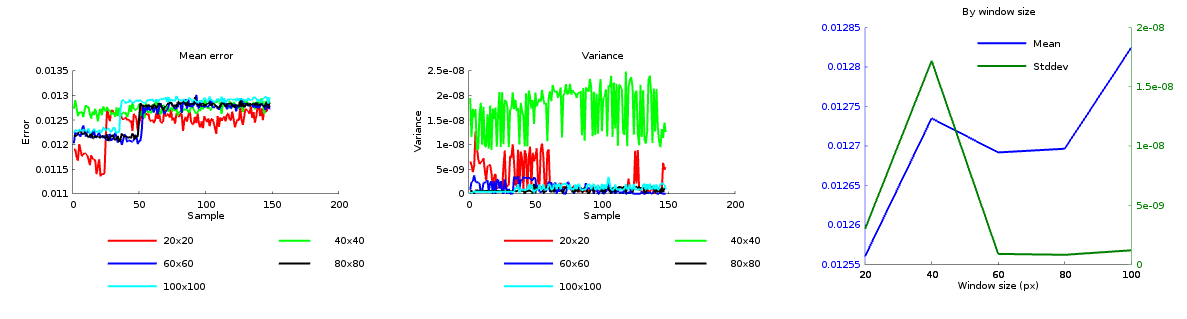
\includegraphics[width=1\textwidth]{figures/plotwindowsizes.png}
  
  \captionof{figure}[Mean and variance: 50cm, varied window sizes]{\label{fig:variedwindow} The error and variance at 50cm for various window sizes.}
\end{figure}

% TODO: Tom : Show plots; Measuring setup;
% TODO: Both : Analysis of plots
\subsection{Noise filtering}

A large issue when implementing the filters was handling the large number of invalid values in the input. In some situations, a majority of the elements were NaN, which obviously makes it hard to draw any conclusions from the data. The \emph{gaussian} and \emph{median} filters from \textbf{OpenCV} work fine  without any modification. The bilateral filter however suffers a segmentation fault when there are NaN values in the input. \par

In order to solve this issue, all NaN-values in the input are set to $10000$ before being passed to the bilateral filter. By the edge preserving property of bilateral filtering, this should reduce the impact they have on the actual filtering process. After the filtering is done, every cell which was set to 10 000 is set to 0; and the mean and variance is calculated on all non-zero elements. \par
Another solution we considered - but did not implement - was to use local median-filtering at each NaN. We deemed this to be a very computationally expensive process, but could possibly yield better results. \par
% TODO: Tom : Implementation, challenges (NAAAN), push code with visible images
% TODO: Marek : Target scene (point 3)
% TODO: Both : Analysis

\section{Results}
% Both : Summary...

\bibliography{References}
\end{document}



%%% Local Variables:
%%% mode: latex
%%% TeX-master: t
%%% End:
